%*******************************************************************************
%********************************* Appendix A **********************************
%*******************************************************************************
\chapter{Appendix A}
\chaptermark{Appendix A}
\label{AppendixA}

\section{Introduction}

Number theory is a field of mathematics that studies integers, it subsumes the branch of combinatorics concerned with counting the number of combinations and permutations of finite sets \citep{Laplace1820}. The Stirling numbers of first, second and third kind play an important role in combinatorial mathematics, they find applications for different analytic and combinatorial problems and they can all be used to express the coefficient of sequences of polynomials. All these numbers are linked by the fact that they can express the number of partitions of a set with $n$ elements into $k$ non-empty non-overlapping subsets. This appendix aims at introducing the Stirling numbers as well as how they can be computed. Also, a presentation of some of their properties as well as the link between them is also provided.

\section{Stirling Numbers of the First Kind}

The Stirling numbers of the first kind are linked to the number of cycles within a finite discrete set. These numbers can be unsigned or signed and are defined by the coefficients of the rising and falling factorials as follows,

\begin{equation} \label{eqnA.1}
x^{(n)} = \prod_{k=0}^{n-1} (x+k) = \sum_{k=0}^{n} \genfrac{[}{]}{0pt}{0}{n}{k} x^{k}.
\end{equation}

The equation \eqref{eqnA.1} defines the rising factorial and its relation with the unsigned Stirling numbers of the first kind, whereas the equation \eqref{eqnA.2} defines the falling factorial along with its relation with the unsigned Stirling numbers of the first kind. The signed Stirling numbers of the first kind are obtained by combining the sign in the sum of \eqref{eqnA.2} with the unsigned Stirling numbers of the first kind.

\begin{equation} \label{eqnA.2}
(x)_{n} = \prod_{k=0}^{n-1} (x-k) = \sum_{k=0}^{n} (-1)^{n-k} \genfrac{[}{]}{0pt}{0}{n}{k} x^{k} 
\end{equation}

The unsigned Stirling numbers of the first kind correspond to the number of permutations of a set of $n$ elements with $k$ disjoint cycles. These numbers can also be computed using the following recurrence relation,

\begin{subequations} \label{eqnA.3}
\begin{align}
\forall (n,k) \in \mathbb{N}^{*} \times \mathbb{N}^{*} ,\, & \genfrac{[}{]}{0pt}{0}{0}{0} = 1 ,\, \genfrac{[}{]}{0pt}{0}{n}{0} = \genfrac{[}{]}{0pt}{0}{0}{n} = 0, \label{eqnA.3a} \\
& \genfrac{[}{]}{0pt}{0}{n+1}{k} = \genfrac{[}{]}{0pt}{0}{n}{k-1} + n \genfrac{[}{]}{0pt}{0}{n}{k}. \label{eqnA.3b}
\end{align}
\end{subequations}

It is possible to show this recurrence relation using either the definition of the Stirling numbers of first kind based on the rising or falling factorials or by using their combinatorial definition based on permutations. The first few Stirling numbers of the first kind are presented within Table \ref{tabA.1}.

\begin{table}[!htbp]
\centering
\caption{Stirling numbers of the first kind.}
\label{tabA.1}
\begin{tabular}{ccccccc}
\toprule
$n \backslash k$ & 0 & 1 & 2 & 3 & 4 & 5 \\
\cmidrule(lr){1-7}
0 & 1 & & & & & \\
1 & 0 & 1 & & & & \\
2 & 0 & 1 & 1 & & & \\
3 & 0 & 2 & 3 & 1 & & \\
4 & 0 & 6 & 11 & 6 & 1 & \\
5 & 0 & 24 & 50 & 35 & 10 & 1 \\
\bottomrule
\end{tabular}
\end{table}

For a fixed value of $n$, the sum of all the Stirling numbers of the first kind over $k$ from $0$ to $n$ yields factorial $n$, which can be computed from the rising factorial with $x$ equal $1$.

\begin{equation} \label{eqnA.4}
\forall n \in \mathbb{N} ,\, \sum_{k=0}^{n} \genfrac{[}{]}{0pt}{0}{n}{k} = n! = \genfrac{[}{]}{0pt}{0}{n+1}{1}
\end{equation}

Using the recursive relation \eqref{eqnA.3}, it is trivial to show that the right side equality of \eqref{eqnA.4} holds.

\begin{figure}[!htbp]
\centering
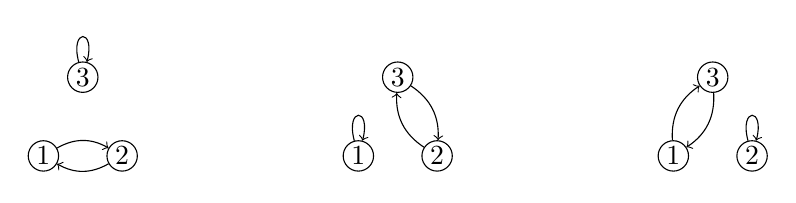
\begin{tikzpicture}
% Set left
\draw (-4,+0) node(n11)[circle,draw=black,inner sep=1pt] {$1$} +(1,0) node(n12)[circle,draw=black,inner sep=1pt] {$2$} +(0.5,1) node(n13)[circle,draw=black,inner sep=1pt] {$3$};
% Set middle
\draw (+0,+0) node(n21)[circle,draw=black,inner sep=1pt] {$1$} +(1,0) node(n22)[circle,draw=black,inner sep=1pt] {$2$} +(0.5,1) node(n23)[circle,draw=black,inner sep=1pt] {$3$};
% Set right
\draw (+4,+0) node(n31)[circle,draw=black,inner sep=1pt] {$1$} +(1,0) node(n32)[circle,draw=black,inner sep=1pt] {$2$} +(0.5,1) node(n33)[circle,draw=black,inner sep=1pt] {$3$};
% Arrows set 1
\draw[->] (n11) edge [bend left] (n12);
\draw[->] (n12) edge [bend left] (n11);
\draw[->] (n13) edge [loop,out=105,in=75,looseness=11] (n13);
% Arrows set 2
\draw[->] (n22) edge [bend left] (n23);
\draw[->] (n23) edge [bend left] (n22);
\draw[->] (n21) edge [loop,out=105,in=75,looseness=11] (n21);
% Arrows set 3
\draw[->] (n33) edge [bend left] (n31);
\draw[->] (n31) edge [bend left] (n33);
\draw[->] (n32) edge [loop,out=105,in=75,looseness=11] (n32);
\end{tikzpicture}
\caption{Cycle representations of the Stirling number of the first kind with $n=3$ and $k=2$.}
\label{figA.1}
\end{figure}

Figure \ref{figA.1} represents the different cycles linked to the Stirling number of the first kind with a set of $n=3$ elements and $k=2$ cycles. The total number of ways to partition the set is $3$. In this case, all three partitions have a cycle composed of $2$ elements and a cycle of a single element.

\section{Stirling Numbers of the Second Kind}

The Stirling numbers of the second kind represent the number of ways to partition a set of $n$ elements into $k$ non-empty non-overlapping subsets. These numbers are the inverse to the Stirling numbers of the first kind. Similarly to the Stirling number of the first kind, they can be computed based on the generating function consisting of the rising and falling factorials \eqref{eqnA.5}, such that,

\begin{equation} \label{eqnA.5}
\forall n \in \mathbb{N} ,\, x^{n} = \sum_{k=0}^{n} \genfrac{\{}{\}}{0pt}{0}{n}{k} (x)_{k} = \sum_{k=0}^{n} (-1)^{n-k}\genfrac{\{}{\}}{0pt}{0}{n}{k} x^{(k)}
\end{equation}

It can be proved that there exists a recurrence relation between the Stirling number of the second kind based on their definition from the falling factorial. The recurrence relation is as follows,

\begin{subequations} \label{eqnA.6}
\begin{align}
\forall (n,k) \in \mathbb{N}^{*} \times \mathbb{N}^{*} ,\, & \genfrac{\{}{\}}{0pt}{0}{0}{0} = 1 ,\, \genfrac{\{}{\}}{0pt}{0}{n}{0} = \genfrac{\{}{\}}{0pt}{0}{0}{n} = 0, \label{eqnA.6a} \\
& \genfrac{\{}{\}}{0pt}{0}{n+1}{k} = k \genfrac{\{}{\}}{0pt}{0}{n}{k} + \genfrac{\{}{\}}{0pt}{0}{n}{k-1}. \label{eqnA.6b}
\end{align}
\end{subequations}

Table \ref{tabA.2} presents the first few Stirling numbers of the second kind which highlights the recurrence relation presented previously.

\begin{table}[!htbp]
\centering
\caption{Stirling numbers of the second kind.}
\label{tabA.2}
\begin{tabular}{ccccccc}
\toprule
$n \backslash k$ & 0 & 1 & 2 & 3 & 4 & 5 \\
\cmidrule(lr){1-7}
0 & 1 & & & & & \\
1 & 0 & 1 & & & & \\
2 & 0 & 1 & 1 & & & \\
3 & 0 & 1 & 3 & 1 & & \\
4 & 0 & 1 & 7 & 6 & 1 & \\
5 & 0 & 1 & 15 & 25 & 10 & 1 \\
\bottomrule
\end{tabular}
\end{table}

There is an explicit formula used to compute the Stirling numbers of the second kind relying on factorials, this formula is as follows,

\begin{equation} \label{eqnA.7}
\genfrac{\{}{\}}{0pt}{0}{n}{k} = \frac{1}{k!} \sum_{i=0}^{k} (-1)^{k-i} \genfrac{(}{)}{0pt}{0}{k}{i} i^{n}.
\end{equation}

The total number of ways to partition a set with $n$ elements into non-empty non-overlapping subsets is defined by the Bell number. Consequently, the $n$-th Bell number $B_{n}$ is equal to the sum of the Stirling numbers of the second kind such that,

\begin{equation} \label{eqnA.8}
\forall n \in \mathbb{N} ,\, \sum_{k=0}^{n} \genfrac{\{}{\}}{0pt}{0}{n}{k} = B_{n}.
\end{equation}

In order to have an idea of the distinct ways to partition a set of $n$ elements into $k$ non-empty non-overlapping subsets, the Figure \ref{figA.2} illustrates all the different partitioning ways with $n=4$ and $k=2$. In this case, there are $6$ possible ways the partition the set of four elements, each one is composed of a subset composed of two elements as well as two subsets with a single element.

\begin{figure}[!htbp]
\centering
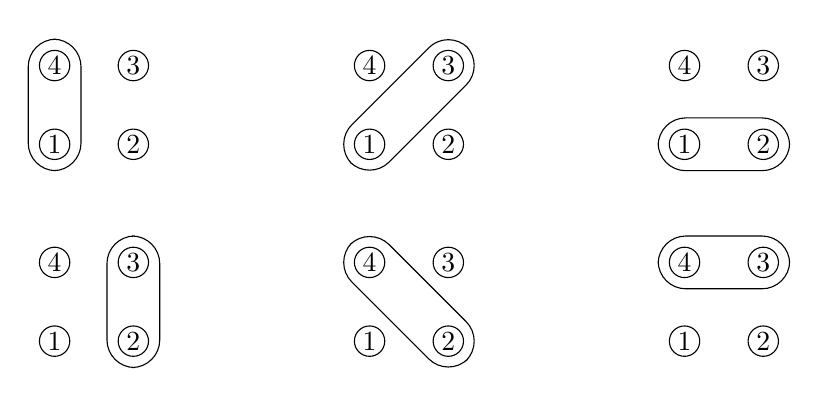
\begin{tikzpicture}[every node/.style={outer sep=8pt}]
% Set top left
\draw (-4,+2.5) node(n11)[circle,draw=black,inner sep=1pt] {$1$} +(1,0) node(n12)[circle,draw=black,inner sep=1pt] {$2$} +(1,1) node(n13)[circle,draw=black,inner sep=1pt] {$3$} +(0,1) node(n14)[circle,draw=black,inner sep=1pt] {$4$};
% Set top middle
\draw (+0,+2.5) node(n21)[circle,draw=black,inner sep=1pt] {$1$} +(1,0) node(n22)[circle,draw=black,inner sep=1pt] {$2$} +(1,1) node(n23)[circle,draw=black,inner sep=1pt] {$3$} +(0,1) node(n24)[circle,draw=black,inner sep=1pt] {$4$};
% Set top right
\draw (+4,+2.5) node(n31)[circle,draw=black,inner sep=1pt] {$1$} +(1,0) node(n32)[circle,draw=black,inner sep=1pt] {$2$} +(1,1) node(n33)[circle,draw=black,inner sep=1pt] {$3$} +(0,1) node(n34)[circle,draw=black,inner sep=1pt] {$4$};
% Set bottom left
\draw (-4,+0) node(n41)[circle,draw=black,inner sep=1pt] {$1$} +(1,0) node(n42)[circle,draw=black,inner sep=1pt] {$2$} +(1,1) node(n43)[circle,draw=black,inner sep=1pt] {$3$} +(0,1) node(n44)[circle,draw=black,inner sep=1pt] {$4$};
% Set bottom middle
\draw (+0,+0) node(n51)[circle,draw=black,inner sep=1pt] {$1$} +(1,0) node(n52)[circle,draw=black,inner sep=1pt] {$2$} +(1,1) node(n53)[circle,draw=black,inner sep=1pt] {$3$} +(0,1) node(n54)[circle,draw=black,inner sep=1pt] {$4$};
% Set bottom right
\draw (+4,+0) node(n61)[circle,draw=black,inner sep=1pt] {$1$} +(1,0) node(n62)[circle,draw=black,inner sep=1pt] {$2$} +(1,1) node(n63)[circle,draw=black,inner sep=1pt] {$3$} +(0,1) node(n64)[circle,draw=black,inner sep=1pt] {$4$};
% Subsets
\path[draw=black,rounded corners=10pt] (n11.south east) -- (n14.north east) -- (n14.north west) -- (n11.south west) -- cycle;
\path[draw=black,rounded corners=10pt] (n21.south) -- (n23.east) -- (n23.north) -- (n21.west) -- cycle;
\path[draw=black,rounded corners=10pt] (n31.south west) -- (n32.south east) -- (n32.north east) -- (n31.north west) -- cycle;
\path[draw=black,rounded corners=10pt] (n42.south east) -- (n43.north east) -- (n43.north west) -- (n42.south west) -- cycle;
\path[draw=black,rounded corners=10pt] (n52.east) -- (n54.north) -- (n54.west) -- (n52.south) -- cycle;
\path[draw=black,rounded corners=10pt] (n64.south west) -- (n63.south east) -- (n63.north east) -- (n64.north west) -- cycle;
\end{tikzpicture}
\caption{Set partitions representing the Stirling number of the second kind with $n=4$ and $k=3$.}
\label{figA.2}
\end{figure}

\section{Lah Numbers}

The Lah numbers, also sometimes called the Stirling numbers of the third kind, represent the number of ways to partition a set of $n$ elements into $k$ non-empty non-overlapping ordered subsets. Similarly to the Stirling number of the first and second kinds, the Lah numbers can be generated using the rising factorial as follows,

\begin{equation} \label{eqnA.9}
x^{(n)} = \sum_{k=1}^{n} \genfrac{\lfloor}{\rfloor}{0pt}{0}{n}{k} (x)_{k}.
\end{equation}

In the same fashion as for the Stirling numbers of the first and second kinds, the Lah numbers are linked to the falling factorial, the relation is as follows,

\begin{equation} \label{eqnA.10}
(x)_{n} = \sum_{k=1}^{n} (-1)^{n-k} \genfrac{\lfloor}{\rfloor}{0pt}{0}{n}{k} x^{(k)}.
\end{equation}

The Lah numbers can be calculated by using the following recurrence relation,

\begin{subequations} \label{eqnA.11}
\begin{align}
\forall (n,k) \in \mathbb{N}^{*} \times \mathbb{N}^{*} ,\, & \genfrac{\lfloor}{\rfloor}{0pt}{0}{0}{0} = 1 ,\, \genfrac{\lfloor}{\rfloor}{0pt}{0}{n}{0} = \genfrac{\lfloor}{\rfloor}{0pt}{0}{0}{n} = 0, \label{eqnA.11a} \\
& \genfrac{\lfloor}{\rfloor}{0pt}{0}{n+1}{k} = (n+k)\genfrac{\lfloor}{\rfloor}{0pt}{0}{n}{k} + \genfrac{\lfloor}{\rfloor}{0pt}{0}{n}{k-1}. \label{eqnA.11b}
\end{align}
\end{subequations}

However, in this case, an explicit formula to compute these numbers exists based on binomial coefficients and factorials exists and is given by,

\begin{equation} \label{eqnA.12}
\genfrac{\lfloor}{\rfloor}{0pt}{0}{n}{k} = \genfrac{(}{)}{0pt}{0}{n-1}{k-1} \frac{n!}{k!}.
\end{equation}

Some properties of the Lah numbers can be proved by recurrence, for example,

\begin{subequations} \label{eqnA.13}
\begin{align}
\forall n \in \mathbb{N}^{*} ,\, & \genfrac{\lfloor}{\rfloor}{0pt}{0}{n}{1} = n!, \label{eqnA.13a} \\
& \genfrac{\lfloor}{\rfloor}{0pt}{0}{n}{n} = 1, \label{eqnA.13b} \\
& \genfrac{\lfloor}{\rfloor}{0pt}{0}{n}{n-1} = n(n-1). \label{eqnA.13c}
\end{align}
\end{subequations}

Finally, Table \ref{tabA.3} presents the first Lah numbers for $n$ less or equal to $5$. The distinct ways to partition a set of $n=3$ elements into $k=2$ non-empty non-overlapping ordered subsets is represented Figure \ref{figA.3}. In this case, there are $6$ different partitions possible, every partition is composed of an ordered subset including two elements and a subset composed of a single element.

\begin{table}[!htbp]
\centering
\caption{Lah numbers.}
\label{tabA.3}
\begin{tabular}{ccccccc}
\toprule
$n \backslash k$ & 0 & 1 & 2 & 3 & 4 & 5 \\
\cmidrule(lr){1-7}
0 & 1 & & & & & \\
1 & 0 & 1 & & & & \\
2 & 0 & 2 & 1 & & & \\
3 & 0 & 6 & 6 & 1 & & \\
4 & 0 & 24 & 36 & 12 & 1 & \\
5 & 0 & 120 & 240 & 120 & 20 & 1 \\
\bottomrule
\end{tabular}
\end{table}

\begin{figure}[!htbp]
\centering
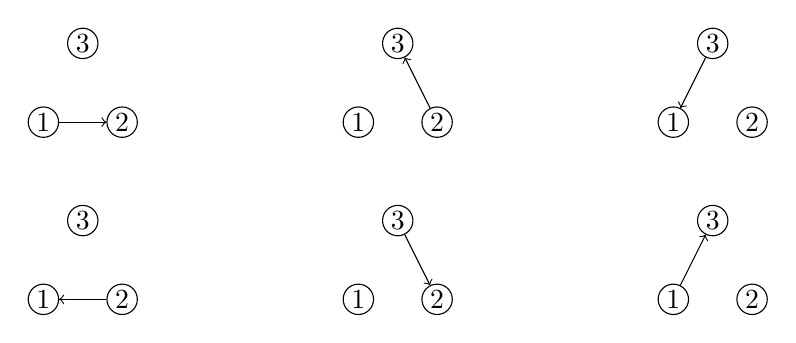
\begin{tikzpicture}
% Set top left
\draw (-4,+2.25) node(n11)[circle,draw=black,inner sep=1pt] {$1$} +(1,0) node(n12)[circle,draw=black,inner sep=1pt] {$2$} +(0.5,1) node(n13)[circle,draw=black,inner sep=1pt] {$3$};
% Set top middle
\draw (+0,+2.25) node(n21)[circle,draw=black,inner sep=1pt] {$1$} +(1,0) node(n22)[circle,draw=black,inner sep=1pt] {$2$} +(0.5,1) node(n23)[circle,draw=black,inner sep=1pt] {$3$};
% Set top right
\draw (+4,+2.25) node(n31)[circle,draw=black,inner sep=1pt] {$1$} +(1,0) node(n32)[circle,draw=black,inner sep=1pt] {$2$} +(0.5,1) node(n33)[circle,draw=black,inner sep=1pt] {$3$};
% Set bottom left
\draw (-4,+0) node(n41)[circle,draw=black,inner sep=1pt] {$1$} +(1,0) node(n42)[circle,draw=black,inner sep=1pt] {$2$} +(0.5,1) node(n43)[circle,draw=black,inner sep=1pt] {$3$};
% Set bottom middle
\draw (+0,+0) node(n51)[circle,draw=black,inner sep=1pt] {$1$} +(1,0) node(n52)[circle,draw=black,inner sep=1pt] {$2$} +(0.5,1) node(n53)[circle,draw=black,inner sep=1pt] {$3$};
% Set bottom right
\draw (+4,+0) node(n61)[circle,draw=black,inner sep=1pt] {$1$} +(1,0) node(n62)[circle,draw=black,inner sep=1pt] {$2$} +(0.5,1) node(n63)[circle,draw=black,inner sep=1pt] {$3$};
% Arrows set 1
\draw[->] (n11) -- (n12);
% Arrows set 2
\draw[->] (n22) -- (n23);
% Arrows set 3
\draw[->] (n33) -- (n31);
% Arrows set 4
\draw[->] (n42) -- (n41);
% Arrows set 5
\draw[->] (n53) -- (n52);
% Arrows set 6
\draw[->] (n61) -- (n63);
\end{tikzpicture}
\caption{Ordered subsets representing the Lah number with $n=3$ and $k=2$.}
\label{figA.3}
\end{figure}

\section{Relations Between the Stirling and Lah Numbers}

The three different combinatorial numbers presented within the previous sections of this appendix are related. It can be seen that they represent a change in basis for polynomial functions as it is pictured by Figure \ref{figA.4}. A Polynomial function can be expressed uniquely with the canonical polynomial basis or with the polynomial basis generated from the rising and the falling factorials. The Figure \ref{figA.4} presents how these numbers connect the three polynomial basis mentioned previously. Therefore, it means that the Stirling number of the first and second kind can be considered as inverses when they form lower triangular matrices whose entries are the Stirling numbers with corresponding row and column indexes. Similarly, as it can be seen Figure \ref{figA.4}, the Lah numbers and the Lah numbers multiplied by $(-1)^{n-k}$ can be seen as inverses when they compose the entries of lower triangular matrices. Finally, since these three combinatorial numbers represent different ways to partition a set of $n$ elements into $k$ subsets being respectively unordered, cyclically ordered and linearly ordered, the following inequalities naturally arise,

\begin{equation} \label{eqnA.14}
\forall (n,k) \in \mathbb{N} \times \mathbb{N} ,\, \genfrac{\{}{\}}{0pt}{0}{n}{k} \leq \genfrac{[}{]}{0pt}{0}{n}{k} \leq \genfrac{\lfloor}{\rfloor}{0pt}{0}{n}{k}
\end{equation}

\begin{figure}[!htbp]
\centering
\begin{tikzpicture}
% Nodes basis
\node (n1) at (0,5) {$x^{n}$};
\node (n2) at (-3,0) {$x^{(n)}$};
\node (n3) at (3,0) {$(x)_{n}$};
% Arrows
\draw[->] (n1) -- node[anchor=north east]{$\genfrac{\{}{\}}{0pt}{0}{n}{k}$} (n3);
\draw (n3) edge[bend right,->] node[anchor=south west]{$(-1)^{n-k}\genfrac{[}{]}{0pt}{0}{n}{k}$} (n1);
\draw[->] (n3) -- node[anchor=south]{$\genfrac{\lfloor}{\rfloor}{0pt}{0}{n}{k}$} (n2);
\draw (n2) edge[bend right,->] node[anchor=north]{$(-1)^{n-k}\genfrac{\lfloor}{\rfloor}{0pt}{0}{n}{k}$} (n3);
\draw[->] (n2) -- node[anchor=north west]{$\genfrac{[}{]}{0pt}{0}{n}{k}$} (n1);
\draw (n1) edge[bend right,->] node[anchor=south east]{$(-1)^{n-k}\genfrac{\{}{\}}{0pt}{0}{n}{k}$} (n2);
\end{tikzpicture}
\caption{Relations between the Stirling and Lah numbers.}
\label{figA.4}
\end{figure}